\apendice{Especificación de diseño}

A continuación se detalla el diseño que se ha generado para realizar Green In House y se detalla en profundidad porque se ha decidido geenrar dicho diseño, que metodologías se han utilizado, que estructar de trabalas y de directorias se ha definido, etc.

\section{Introducción}
Realizar un buen diseño de las especificaciones del sistema supone una enorme diferencia a la hora de realizar la codificación y el posterior mantenimiento y crecimiento de la aplicación. Si se parte de un mal diseño, habrá que ir haciendo apaños continuamente para poder ir incluyendo funcionalidades. Por contra, si se parte de un buen diseño, que esté pensado para ser modular y crecer continuamente, la inclusión de nuevas funcionalidades se realizará de manera sencilla y orgánica, si necesidad de generar apaños extraños o refactorizar el código de la aplicación completa.

\section{Diseño de datos}

A continuación se detalla la estructura que tiene cada tabla de la base de datos y se especifica como se interrelacionan entre ellas. 

    \subsection{Tablas de la base de datos e interrelación entre ellas}
        Las tablas que se han diseñado para utilizar en Green In House y las interrelacciones que se han creado entre ellas son las siguientes:
        \begin{itemize}
            \item \textbf{tipos\_plantas}
            \begin{itemize}
                \item tipo\_planta \texttt{\{String\}} \textbf{PK}: El tipo de planta.
                \item descripcion\_planta \texttt{\{String\}}: Descripción del tipo de planta.
            \end{itemize}
            \item \textbf{plantas}
            \begin{itemize}
                \item nombre\_planta \texttt{\{String\}} \textbf{PK}: El nombre de la planta.
                \item tipo\_planta \texttt{\{String\}} \textbf{FK} de \textit{tipos\_plantas.tipo\_planta}: El tipo de la planta.
                \item fecha\_plantacion \texttt{\{Timestamp\}}: La fecha de plantación de la planta.
                \item fecha\_marchitacion \texttt{\{Timestamp\}}: La fecha de marchitación de la planta.
            \end{itemize}
            \item \textbf{sensores}:
            \begin{itemize}
                \item tipo\_sensor \texttt{\{Enum type\}} \textbf{PK}: El tipo de sensor.
                \item zona\_sensor \texttt{\{Enum type\}} \textbf{PK}: La zona del sensor.
                \item numero\_sensor \texttt{\{Integer\}} \textbf{PK}: El número del sensor.
                \item modelo\_sensor \texttt{\{Enum type\}}: El modelo del sensor.
                \item nombre\_sensor \texttt{\{String\}}: El nombre del sensor para reconocerle fácilmente.
                \item direccion\_lectura \texttt{\{String\}}: La dirección de lectura del sensor.
                \item patilla\_0\_lectura \texttt{\{Integer\}}: Pin 0 de lectura del sensor.
                \item patilla\_1\_lectura \texttt{\{Integer\}}: Pin 1 de lectura del sensor.
                \item patilla\_2\_lectura \texttt{\{Integer\}}: Pin 2 de lectura del sensor.
                \item patilla\_3\_lectura \texttt{\{Integer\}}: Pin 3 de lectura del sensor.
                \item unidad\_medida\_0 \texttt{\{Enum type\}}: Unidad de medida 0 para los datos recogidos por el sensor.
                \item unidad\_medida\_1 \texttt{\{Enum type\}}: Unidad de medida 1 para los datos recogidos por el sensor.
                \item unidad\_medida\_2 \texttt{\{Enum type\}}: Unidad de medida 2 para los datos recogidos por el sensor.
                \item unidad\_medida\_3 \texttt{\{Enum type\}}: Unidad de medida 3 para los datos recogidos por el sensor.
                \item fecha\_creacion \texttt{\{Timestamp\}}: Fecha de creación del sensor.
                \item fecha\_eliminacion \texttt{\{Timestamp\}}: Fecha de eliminación del sensor.
            \end{itemize}
            \item \textbf{sensores\_plantas}
            \begin{itemize}
                \item id\_ \texttt{\{Integer\}} \textbf{PK}: Un identificador del registro de unión de sensor y planta.
                \item tipo\_sensor \texttt{\{Enum type\}} \textbf{FK} de \textit{sensores.tipo\_sensor}: El tipo de sensor.
                \item zona\_sensor \texttt{\{Enum type\}} \textbf{FK} de \textit{sensores.zona\_sensor}: La zona del sensor.
                \item numero\_sensor \texttt{\{Integer\}} \textbf{FK} de \textit{sensores.numero\_sensor}: El número del sensor.
                \item nombre\_planta \texttt{\{String\}} \textbf{FK} de \textit{ plantas.nombre\_planta}: El nombre de la planta asociada al sensor.
                \item fecha\_asociacion \texttt{\{Timestamp\}}: Fecha de asociación del sensor a la planta.
                \item fecha\_anulacion \texttt{\{Timestamp\}}: Fecha de anulación de la asociación del sensor a la planta.
            \end{itemize}
            \item \textbf{registros\_sensores}
            \begin{itemize}
                \item id\_ \texttt{\{Integer\}} \textbf{PK}: El identificador del registro del sensor.
                \item tipo\_sensor \texttt{\{Enum type\}} \textbf{FK} de \textit{sensores.tipo\_sensor}: El tipo de sensor.
                \item zona\_sensor \texttt{\{Enum type\}} \textbf{FK} de \textit{sensores.zona\_sensor}: La zona del sensor.
                \item numero\_sensor \texttt{\{Integer\}} \textbf{FK} de \textit{sensores.numero\_sensor}: El número del sensor.
                \item valor \texttt{\{Float\}}: El valor registrado por el sensor.
                \item unidad\_medida \texttt{\{Enum type\}}: La unidad de la medida.
                \item fecha \texttt{\{Timestamp\}}: La fecha del registro.
            \end{itemize}
            \item \textbf{consejos\_plantas}
            \begin{itemize}
                \item descripcion \texttt{\{String\}}: Una descripción del consejo.
                \item nombre\_elemento \texttt{\{String\}} \textbf{PK} \textbf{FK} de \textit{ plantas.nombre\_planta}: El nombre del elemento que se refiere al consejo.
                \item zona\_consejo \texttt{\{Enum type\}} \textbf{PK}: La zona del sensor.
                \item tipo\_medida \texttt{\{Enum type\}} \textbf{PK}: El tipo de medida.
                \item unidad\_medida \texttt{\{Enum type\}}: La unidad de la medida.
                \item valor\_minimo \texttt{\{Float\}}: El valor mínimo de la medida.
                \item valor\_maximo \texttt{\{Float\}}: El valor máximo de la medida.
                \item horas\_minimas \texttt{\{Integer\}}: Las horas mínimas de la medida.
                \item horas\_maximas \texttt{\{Integer\}}: Las horas máximas de la medida.
            \end{itemize}
            \item \textbf{consejos\_tipos\_plantas}
            \begin{itemize}
                \item descripcion \texttt{\{String\}}: Una descripción del consejo.
                \item nombre\_elemento \texttt{\{String\}} \textbf{PK} \textbf{FK} de \textit{tipos\_plantas.tipo\_planta}: El nombre del elemento que se refiere al consejo.
                \item zona\_consejo \texttt{\{Enum type\}} \textbf{PK}: La zona del sensor.
                \item tipo\_medida \texttt{\{Enum type\}} \textbf{PK}: El tipo de medida.
                \item unidad\_medida \texttt{\{Enum type\}}: La unidad de la medida.
                \item valor\_minimo \texttt{\{Float\}}: El valor mínimo de la medida.
                \item valor\_maximo \texttt{\{Float\}}: El valor máximo de la medida.
                \item horas\_minimas \texttt{\{Integer\}}: Las horas mínimas de la medida.
                \item horas\_maximas \texttt{\{Integer\}}: Las horas máximas de la medida.
            \end{itemize}
        \end{itemize}

    \subsubsection{Utilización de un sistema de fechas}
    Para no violar la integridad referencial de los datos de la base de datos, no se permite borrar las instancias de los datos una vez grabadas. Para poder marcarlas como eliminadas se ha empleado un sistema de fechas, el cual determina cuando se creó la instancia y cuando se declaró como eliminada.

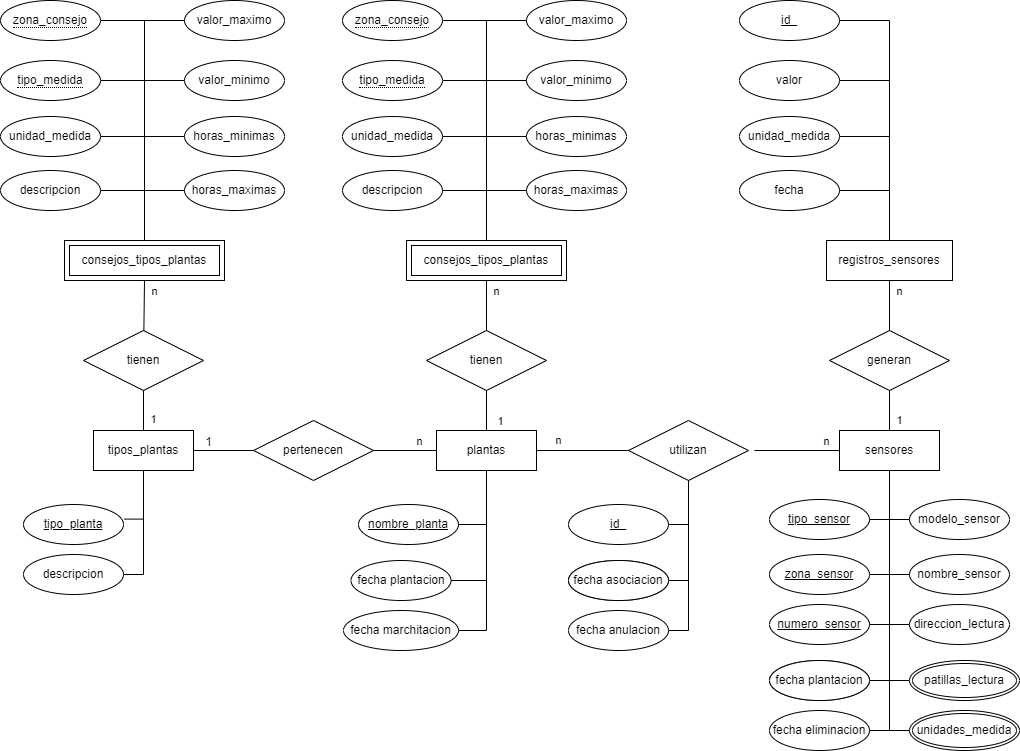
\includepdf[pages=1,fitpaper]{diagrama_entidad_relaccion}  

\section{Diseño procedimental}
Todas las siguientes entidades, las cuales son con las que trabaja Green In House para poder funcionar, siguen la misma estructura de clases, la cual se detalla a continuación. La única diferencia que hay entre estas entidades se debe a los atributos que contiene cada entidad, acorde a lo especificado en el diseño de datos, y a como se utilizan esos atributos para filtrar los objetos en los métodos get y list, utilizados para recuperar objetos de la base de datos. El método post y create se utiliza para crear los objetos en la base de datos. El método update se utiliza para actualizar los datos de los objetos en la base de dar y el método unsubscribe se utilizar para dar de baja dichos objetos, almacenando la fecha en que se dieron de baja.
\begin{itemize}
        \item Sensores
        \item Registros Sensores
        \item Plantas
        \item Tipos Plantas
        \item Sensores Plantas
        \item Consejos Plantas
        \item Consejos Tipo Plantas
    \end{itemize}
    
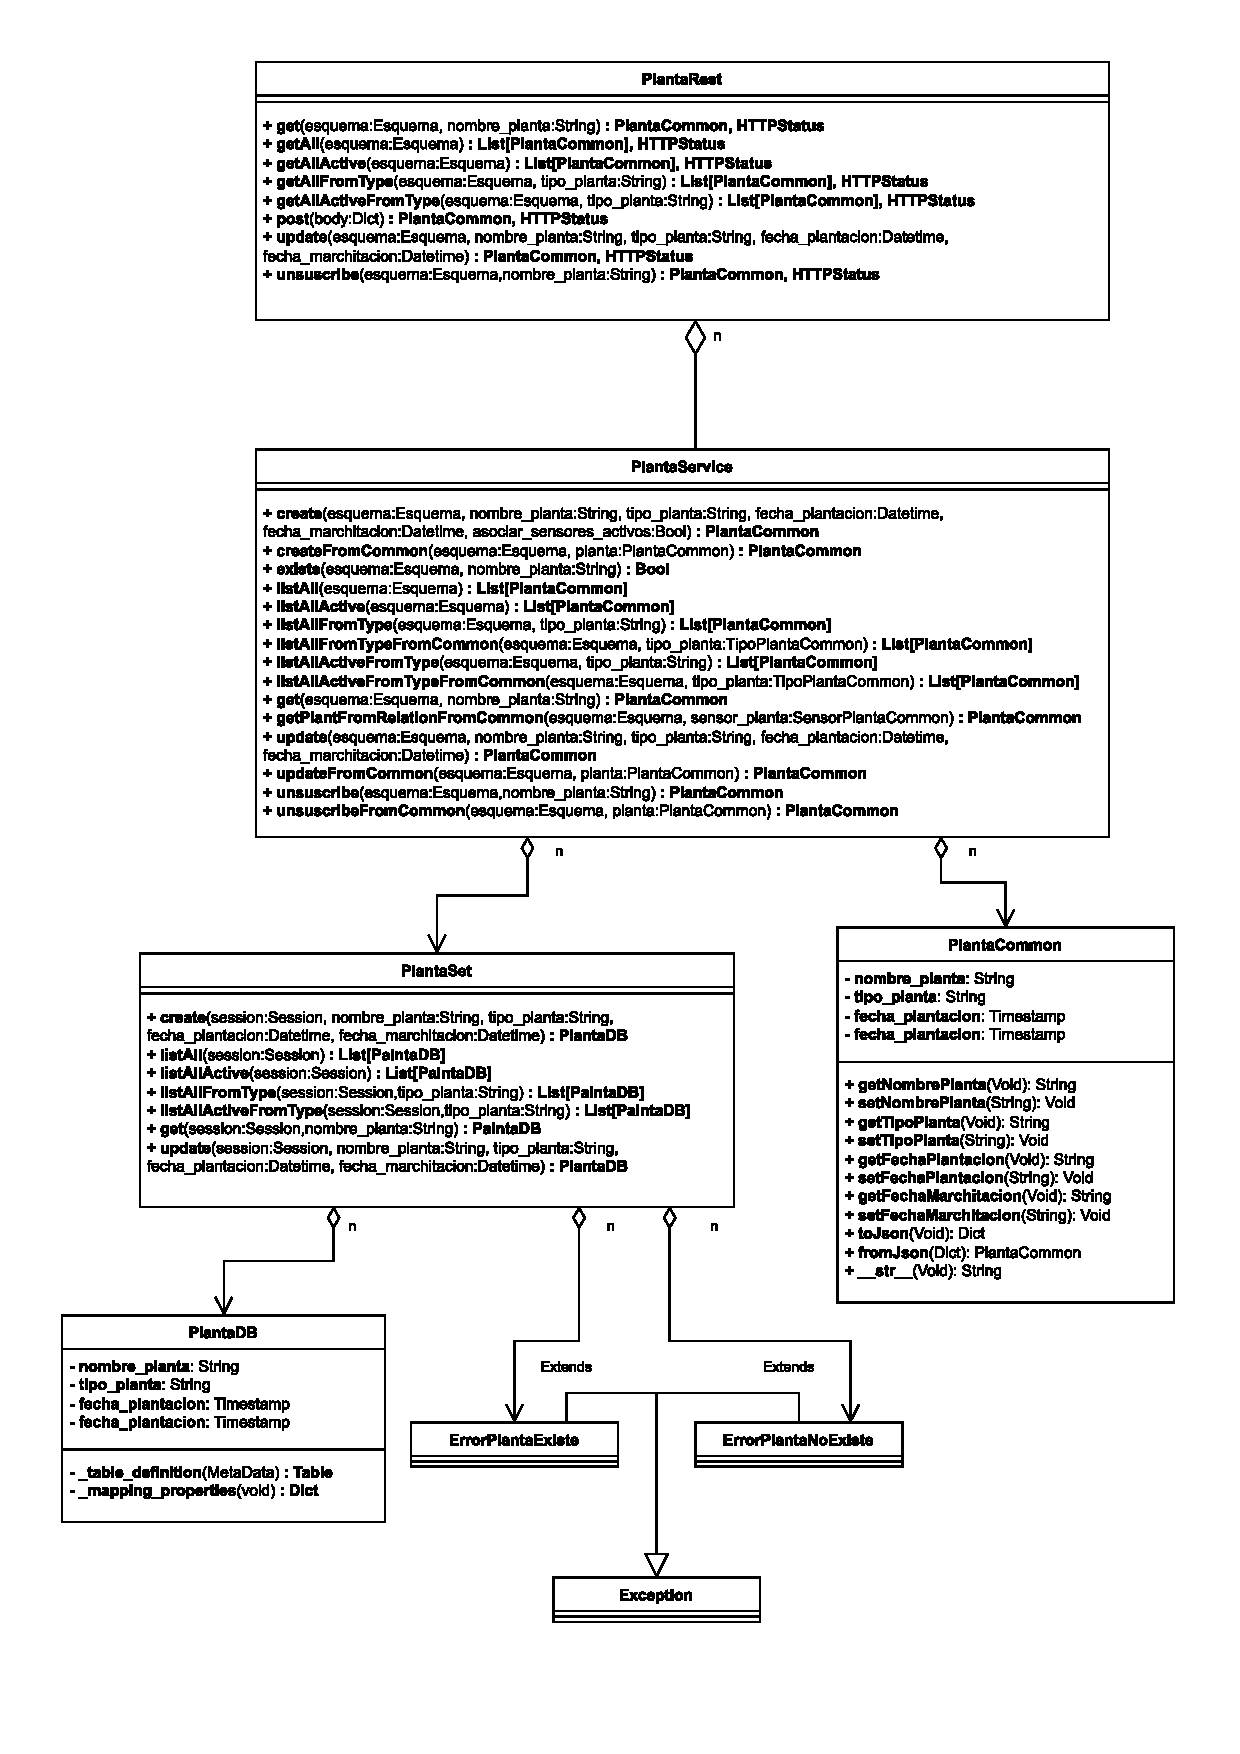
\includepdf[pages=1,fitpaper]{diagrama_de_clases}  


%TODO clases de sensor electronico

%TODO pantalla tactil servicos wifi


El usuario siempre va a interactuar con el sistema a través del API REST, ya sea desde la aplicación móvil haciendo consultas a la API REST, como desde un cliente API REST estilo postman o el propio Swager que recupere los objetos JSON para leerlos. Por lo tanto, la secuencia del flujo de consultas siempre va a ser muy similar al que se detalla en el ejemplo de acontinuación. En este ejemplo se aprecia como el usuario utiliza un método de la API REST, el cual utiliza un método de la capa de servicos, el cual a su vez hace uso de un método del manejador de la base de datos para dicha clase. Esto devuelve una instancia de la base de datos en forma de objeto, del cual se extraen sus atributos para generar un objeto del tipo common, con el que poder trabajar en la applicación de manera segura, sin miedo a que sea modificado por error y esto realice algún cambio en los datos de la instanciar al hacer el commit de alguna transacción en curso.

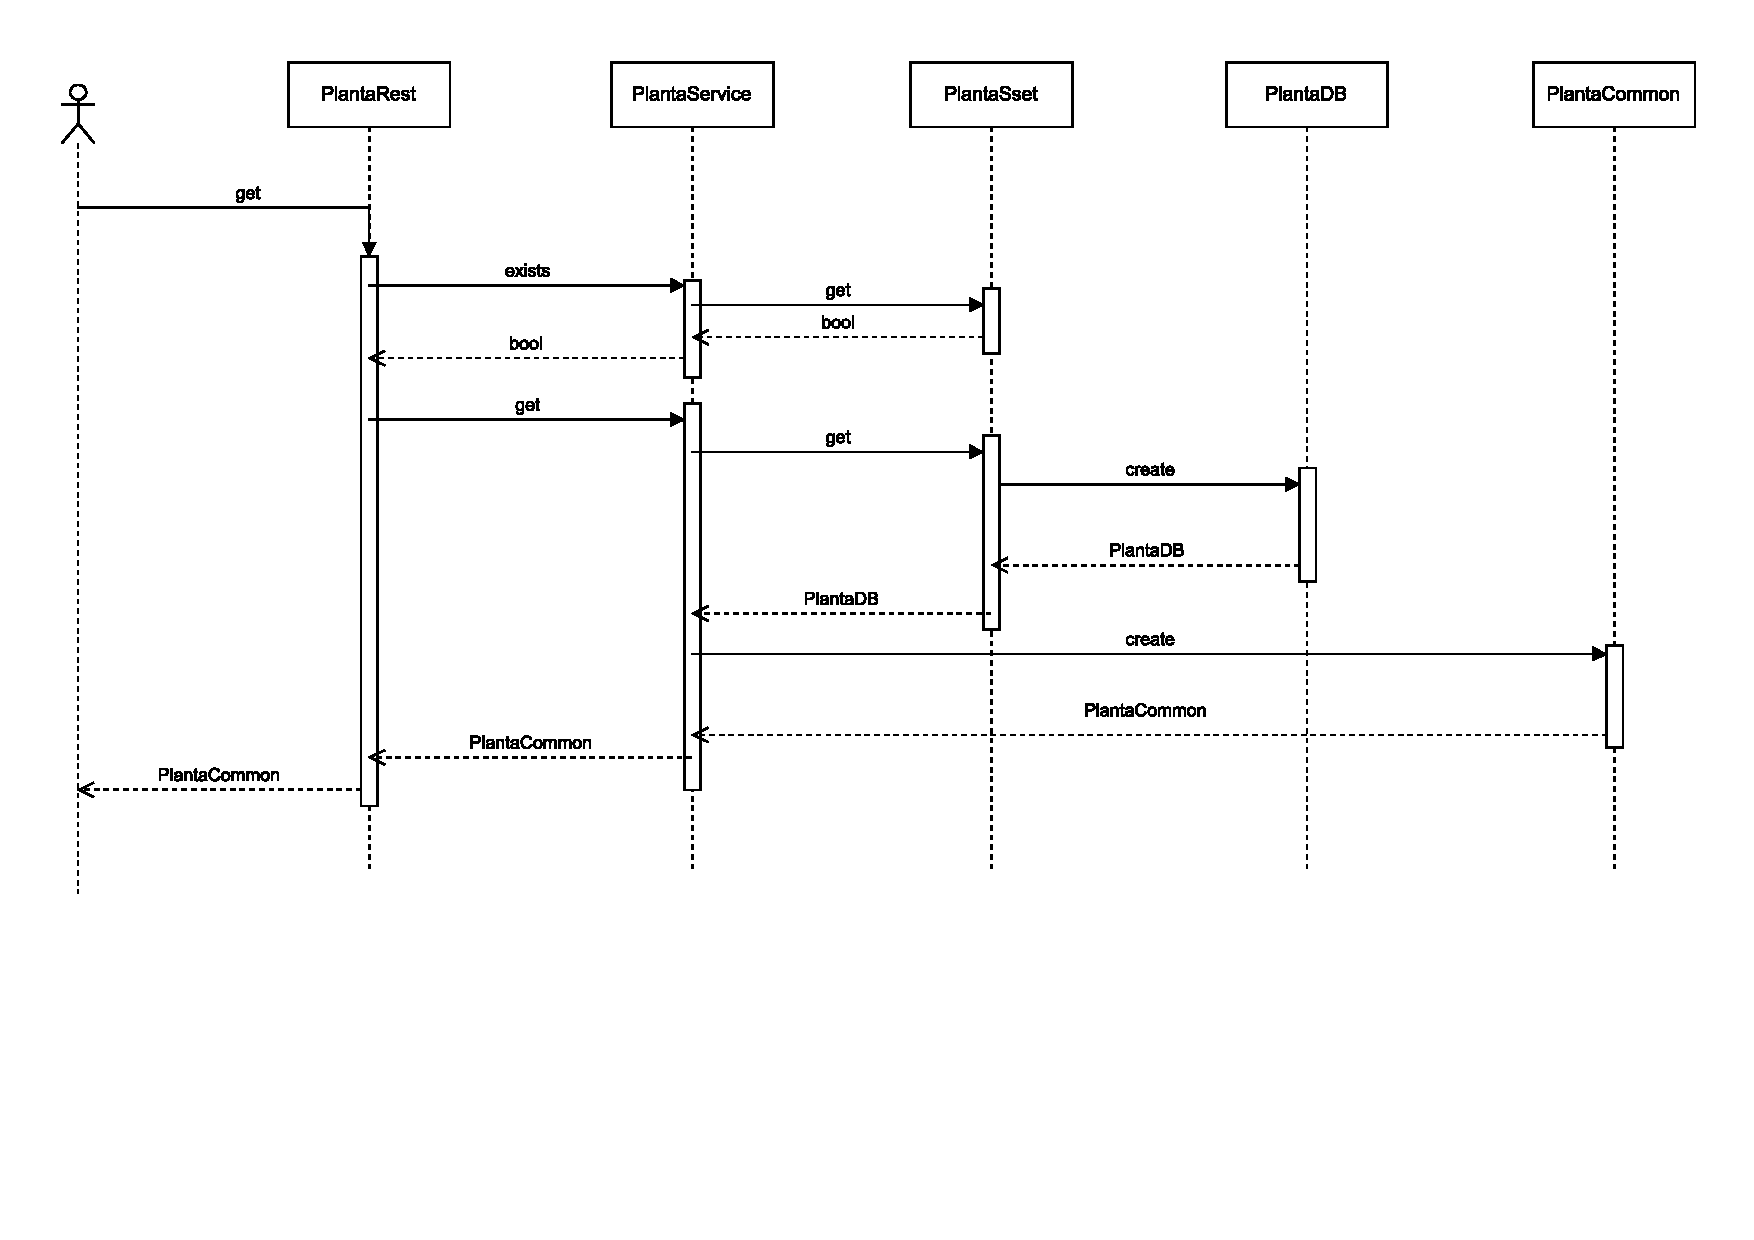
\includepdf[pages=1,fitpaper]{diagrama_de_secuencia}  

%TODO Generar diagrama de como sensor backend encapsula sensor electronico que usa factoria para crear el tipo correspondiente

%TODO Generar diagrama de pantalla como usa servicios para definir las credenciales de red

\section{Diseño arquitectónico}
Para poder desarrollar la arquitectura de Green In House de manera eficiente y con amplias posibilidades de crecimiento y reutilización, se ha recurrido a la utilización de patrones de diseño. Para la realización de la estructura inicial de Green In House separando las funcionalidades en diferentes capas y servicios, reutilicé la estructura básica de la práctica final de la asignatura "Diseño y mantenimiento del software". De esta práctica reutilicé y modifiqué según mis necesidades, algunos archivos de código fuente originalmente desarrollados por Jesús Alonso Abad, para definir los servicios básicos de configuración de directorios de la base de datos y de la API REST, así como la instalación de dependencias declaradas para cada entorno virtual, adaptándolos al código y estructura de Green In House.

    \subsection{Patrón de diseño MVC (Modelo-Vista-Controlador)}
    El patrón de diseño Modelo-Vista-Controlador (MVC) se ha utilizado en Green In House para separar la lógica de la aplicación en tres componentes principales: el Modelo, la Vista y el Controlador. 
        \subsubsection{Modelo} 
        Gestiona los datos y las reglas de negocio de Green In House. Representa la información con la que trabaja y se encarga de acceder a los datos, almacenarlos y procesarlos. Estas clases están alojadas con la siguiente estructura:
        \begin{itemize}
            \item \textbf{/GreenInHouse/db/GreenInHouseBackend.sqlite3.db :} Archivo que almacena la base de datos SQLite3. Para manejar las consultas a este archivo desde Green In House se utiliza SQLAlchemy.
            \item \textbf{components/backend/backend/data :} En este directorio se almacenan las clases de datos del backend y sus clases manejadoras encargadas de recuperarlas de la base de datos y grabarlas de nuevo.
            \begin{itemize}
                \item \textbf{\texttt{./db/results :}} clases de datos de las tablas almacenadas en la base de datos y de cada una de sus instancias.
                \item \textbf{\texttt{./db/resultsets :}} clases de datos manejadoras de las tablas de la base de datos y de sus instancias.
                \item \textbf{\texttt{./db/exc :}} clases de excepción propias lanzadas durante problemas con la base de datos.
                \item \textbf{\texttt{./db/esquema.py :}} clase que define el esquema principal de la base de datos.
                \item \textbf{\texttt{./electronic :}} clases de datos utilizadas para generar objetos a través de los cuales interactuar con los sensores de la aplicación.
                \item \textbf{\texttt{./util :}} clases de datos genéricos de los sensores electrónicos
            \end{itemize}
            \item \textbf{components/common/common/data/util :} clases de datos genéricas de los objetos utilizados en Green In Hosue desligadas de su representación en la base de datos. Estas clases son utilizadas para poder compartir por la aplicación los objetos recuperados de la base de datos, sin riesgo a que sean modificados por error y eso repercuta en la base de datos.
        \end{itemize}  
        
        \subsubsection{Vista}
        Es la representación visual de los datos que maneja el modelo. Se encarga de mostrar la información al usuario de una forma entendible. Estas clases están alojadas con la siguiente estructura:
        \begin{itemize}
            \item \textbf{\texttt{components/backend/backend/presentacion/rest :}}clases que definen los \textit{endpoints} a través de los que otros sistemas interactúan con Green In House mediante el uso de su servidor API REST.
            \item \textbf{\texttt{components/backend/backend/openapi/spec.ymlt :}} clase definida según la especificación OpenAPI que de define como tiene que funcionar internamente el servidor API REST 
            \item \textbf{\texttt{components/frontend/frontend/app/rpi :}} clases que definen y gestionan la aplicación multiventana desplegada en la pantalla táctil de Green In House.
            \item \textbf{Aplicación Flutter :} aplicación multiplataforma que gestiona como interactuar con Green In House desde un dispositivo móvil.
        \end{itemize}
        
        \subsubsection{Controlador} 
        Es el intermediario entre la vista y el modelo. Gestiona la interacción del usuario con la vista, procesa las acciones del usuario y actualiza el modelo cuando es necesario. Estas clases están alojadas con la siguiente estructura:
        \begin{itemize}
            \item \textbf{\texttt{components/backend/backend/service :}} clases que definen los servicios a través de los cuales se utilizan de manera sencilla y cómoda los objetos de la aplicación sin necesidad de saber como está contruida internamente ni como son las interrelaciones entre los objetos. 
            \item \textbf{\texttt{components/backend/bin :}} scripts que gestionan el lanzamiento de los servicios de backend de Green In House, como el servidor API REST, la lectura de la base de datos, la lectura de los sensores y la lectura periódica de los sensores activos.
            \item \textbf{\texttt{componentes/backend/backend/config :}} clases de configuración de como lanzar los servicios de backend.
            \item \textbf{\texttt{components/common/common/service :}} clases que definen y gestionan servicios comunes como la gestión de la conectividad WiFi.
            \item \textbf{\texttt{components/frontend/bin :}} scripts que gestionan el lanzamiento de los servicios de frontend de Green In House, como la aplicación de interacción de la pantalla táctil de la maceta.
            \item \textbf{\texttt{config :}} archivos de configuración de como lanzar los servicios de backend.
            \item \textbf{\texttt{init :}} archivos de configuración de como lanzar durante el arranque de la raspberry los servicios de frontend de Green In House.
            \item \textbf{\texttt{scripts :}} scripts que gestionan la instalación de Green In House y sus entornos virtuales y dependencias, la configuración del sistema y el lanzamiento y la parada de los servicios de backend y frontend.
        \end{itemize}
        
    \subsection{Patrón de diseño Adaptador:}
        Se implementa la clase SensorElectronico, la cual utiliza el patrón de diseño Adaptador, implementando una interfaz común de los métodos para realizar la lectura de los sensores. De esta interfaz heredan el resto de clases de sensores electrónicos del sistema (SensorElectronicoDHT11, SensorElectronicoMCP3008, etc), los cuales implementan los métodos de lectura suministrados, acorde a lo necesario para leer su correspondiente sensor electrónico del mundo real.
        A su vez, la clase SensorElectronicoMCP3008 se implementa como un adaptador de todos los módulos de sensores que necesiten hacer uso del módulo de conversión analógico digital MCP3008 para ser leídos por las Raspberry Pi, definiendo su método de comunicación y sus patillas a través de las cuales realizar las lecturas. 
    %TODO diagrama
    
    \subsection{Patrón de diseño Factoría}
        En la clase FactoriaSensorElectronico se utiliza el patrón de diseño Factoría. Esta clase recibe el modelo de sensor que se quiere leer y los datos de las patillas que se van a utilizar para leerle. Con esos datos se encarga de generar un objeto SensorElectronico con la implementación correspondiente para poder leer dicho sensor.
    %TODO diagrama
    
    \subsection{Patrón de diseño Estrategia}
        En la clase SensorBackend se utiliza el patrón de diseño Estrategia para adaptarse al contexto suministrado, el cual son los datos almacenados de un sensor en la base de datos. Mediante el uso de dicho contexto, se llama a la factoría de sensores electrónicos para que devuelva un objeto SensorElectronico capaz de interactuar con el sensor real del modelo especificado a través de las patillas de comunicación especificadas. 
    %TODO diagrama
    
    \subsection{Patrón de diseño Plantilla}
        En la clase SensorBackend se utiliza el patrón de diseño Plantilla al definir de manera general la lógica que permite leer dicho sensor electrónico, generar un registro del valor leído por el sensor y almacenar dicho registro en la base de datos. Para ello se utilizan los métodos suministrados por el adaptador SensorElectronico, los cuales son sobreescritos es su clase específica por su correspondiente implementación específica.
    %TODO diagrama
    
    \subsection{Partón de diseño Fachada}
        Se implementa una fachada mediante una capa de servicios que permite manejar de manera simple y cómoda las clases de Green In House y su interacción con la base de datos, sin necesidad de conocer como está programado y diseñado internamente.
        Se implementa una fachada mediante una capa manejadora de la API REST, la cual permite a aplicaciones externas hacer un uso sencillo del sistema y los datos almacenados en él, sin la necesidad de conocer como está programado y diseñado internamente.
    %TODO diagrama
    
    \subsection{Partón de diseño Singleton}
        Durante el lanzamiento del servidor API REST se define una única instancia de aplicación, la cual se almacena de manera global mediante el uso de Flask. Esta instancia de aplicación Flask se recupera cuando se hace uso de los métodos de la API REST para recuperar el directorio de la base de datos y pasárselo a la capa de servicios para que trabaje con él.
    %TODO diagrama

\section{Diseño 3D}

Para la realización del prototipo se ha realizado un diseño de modelado 3D de la maceta de Green In House preparada para albergar la planta, la raspberri y la pantalla tactil. Estos archivos han sido diseñados por Yeray Pescador Calleja y se encuentran accesibles en el repositorio de Green In House \cite{GreenInHouse:repo:Maceta}, en el apartado \texttt{/cad3D/maceta}. En las imágenes \ref{fig:maceta1}, \ref{fig:maceta2} y \ref{fig:maceta3} puede apreciarse como es el diseño 3D de la maceta educativa de Green In House..
\imagen{maceta1}{captura de pantalla 1 del modelo 3D de Green In House.}{.7}
\imagen{maceta2}{captura de pantalla 2 del modelo 3D de Green In House.}{.7}
\imagen{maceta3}{captura de pantalla 3 del modelo 3D de Green In House.}{.7}



